\documentclass{beamer}

\usepackage[french]{babel}
\usepackage[T1]{fontenc}
\usepackage[utf8]{inputenc}

\usepackage{graphicx}

\title{Lancer de rayon}
\subtitle{Première partie}
\author{Simon Chopin et Marie-Morgane Paumard}
\date{26 novembre 2013}

\usetheme{CambridgeUS}
\usecolortheme{rose}

\begin{document}

\begin{frame}
	\titlepage
\end{frame}

\section{Introduction}

\begin{frame}{Introduction}
\begin{alertblock}{Définition}
Le lancer de rayon est une technique de synthèse d'image. Il s'agit de calculer
les trajectoiress des rayons lumineux depuis la caméra jusqu'à l'objet, puis de
l'objet jusqu'à la source.
\end{alertblock}

\begin{center}
  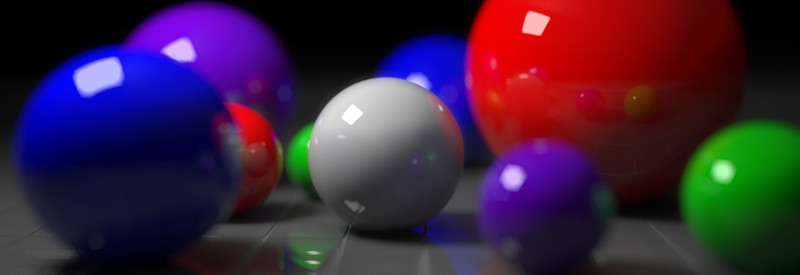
\includegraphics[scale=0.2]{img/intro.jpg}
\end{center}

\begin{block}{Historique}
  \begin{description}
    \item[Raycasting (1968)] Lancer un rayon pixel par pixel et trouver l'objet
le plus proche.
    \item[\textsc{Whitted} (1979)] Génération des rayons : ombre, réflexion et
réfraction.
  \end{description}
\end{block}

\end{frame}

\begin{frame}{Table des matières}
	\tableofcontents
\end{frame}

\section{1}

\section{2}

\section{Améliorations}
\begin{frame}{Gestion de plusieurs sources}

\end{frame}

\begin{frame}{Objets non sphériques}
\end{frame}

\begin{frame}{Ombres portées}
\end{frame}

\begin{frame}{Gestion des matériaux : la réfraction}
\end{frame}

\begin{frame}{Gestion des matériaux : la réflexion}
\end{frame}

\begin{frame}{Autres améliorations}
\end{frame}

\section{Conclusion}
\begin{frame}{Conclusion}
\end{frame}

\end{document}
